\documentclass{article}
\usepackage{amsmath}
\usepackage{amssymb}
\usepackage[pdftex]{graphicx}
\usepackage[]{mcode}
\usepackage{pgfplots}

\pdfpagewidth 8.5in
\pdfpageheight 11in
\topmargin -1in
\headheight 0in
\headsep 0in
\textheight 8.5in
\textwidth 6.5in
\oddsidemargin 0in
\evensidemargin 0in 
\headheight 50pt
\headsep 0in
\footskip .75in

\title{STA 601 - Lab 3}
\author{Kedar Prabhudesai}
\date{September 19, 2013}

\begin{document}
\maketitle
\noindent \underline{Data Model:} \\
\indent $y|N,\beta \sim Binomial(N,\beta)$\\
\noindent \underline{Priors:} \\
\indent $N \sim Beta(1,1)$\\
\indent $\beta \sim Poisson(\lambda)$\\
\noindent \underline{Given:}\\
\indent $y=20$, $\lambda=25.$\\

\begin{enumerate}
\item \underline{Joint Posterior:}
\begin{align*}
p(N,\beta|y) &\propto p(y|N,\beta)p(N,\beta)\\
&\propto p(y|N,\beta)p(N)p(\beta)\\
&\propto \binom{N}{20}\beta^{20}(1-\beta)^{N-20} \times \frac{25^{N}}{N!}exp(-25)\\
&\propto \frac{N!}{(N-20)!20!} \beta^{20}(1-\beta)^{N-20} \times \frac{25^{N}exp(-25)}{N!} \times \frac{25^{-20}}{25^{-20}}\\
\therefore p(N,\beta|y) &\propto \frac{\beta^{20}[25(1-\beta)]^{N-20}}{(N-20)!}\\
\end{align*}

\noindent Since this is a non-standard distribution, we will find the Full Conditionals.

\item \underline{Posterior Full Conditionals:}
\begin{align*}
p(N|\beta,y) &\propto \frac{[25(1-\beta)]^{N-20}}{(N-20)!} \times \frac{exp^{-25(1-\beta)}}{exp^{-25(1-\beta)}}\\
&\propto \frac{[25(1-\beta)]^{N-20}exp^{-25(1-\beta)}}{(N-20)!}\\
\therefore N|\beta,y &\sim Poisson(25(1-\beta))
\end{align*}
This is a shifted Poisson. Hence, we need to add 20 to the samples drawn from this distribution.\\
\begin{align*}
p(\beta|N,y) &\propto \frac{\beta^{20}[25(1-\beta)]^{N-20}}{(N-20)!}\\
&\propto \beta^{20}(1-\beta)^{N-20}\\
\therefore \beta|N,y &\sim Beta(21,N-19).
\end{align*}

\pagebreak
\item To sample from the Joint Posterior we can do Gibbs Sampling:\\
\begin{itemize}
\item Select, $\beta^{(0)}=0.05,$
\item Draw, $N^{(1)} \sim p(N|\beta^{(0)},y)$
\item Draw, $\beta^{(1)} \sim p(\beta|N^{(1)},y)$
\item Hence, we get $\{N^{(1)},\beta^{(1)}\}$.
\item Repeat.
\end{itemize}

\item \underline{Trace Plot for first 10 Samples of Gibbs Sampler.}\\
\begin{center}
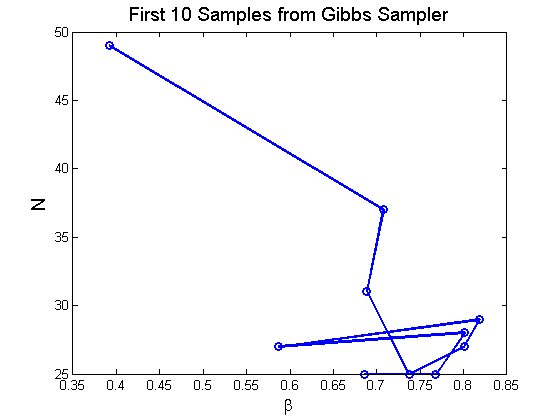
\includegraphics[scale=0.5]{First10Samples.png}\\
\end{center}

\item \underline{Credible Interval:}\\
90\% Posterior Credible Interval for $\beta:[0.54,0.97]$. Magenta line is the mean and red lines represent 90\% Credible Limits.\\
\begin{center}
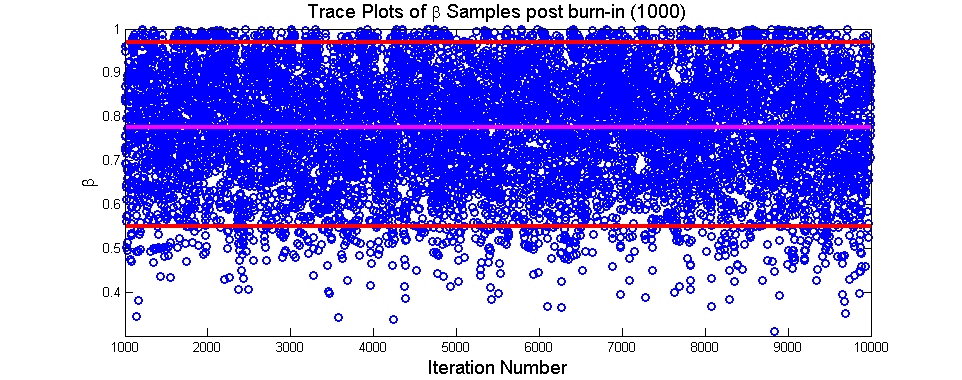
\includegraphics[scale=0.5]{BetaCredIntervals.png}\\
\end{center}

\item \underline{$P(N=20)$} = 0.07 (post burn-in).\\
\end{enumerate}

\pagebreak
\noindent {\Large\underline{\textbf{Appendix:}}}\\
\lstinputlisting{C:/Users/ksp6/Documents/Classes/2013-Fall/STA601-BayesAndModStats/labs/lab3/sta601_ksp6_Lab3.m}

\end{document}